\documentclass[11pt,a4paper]{article}

\usepackage[margin=1in]{geometry}
\usepackage[T1]{fontenc}
\usepackage[utf8]{inputenc}
\usepackage{lmodern}
\usepackage{graphicx}
\usepackage{booktabs}
\usepackage{longtable}
\usepackage{tabularx}
\usepackage{array}
\usepackage{float}
\usepackage{hyperref}
\usepackage{amsmath}
\usepackage{siunitx}
\usepackage{enumitem}
\usepackage{xcolor}
\usepackage{caption}

\hypersetup{
  colorlinks=true,
  linkcolor=blue!50!black,
  urlcolor=blue!50!black
}

\setlength{\parindent}{0pt}
\setlength{\parskip}{0.6em}
\setlength{\tabcolsep}{4pt}
\emergencystretch=2em
\setlist[itemize]{leftmargin=1.5em, itemsep=0.2em, topsep=0.2em}
\renewcommand{\arraystretch}{1.15}
\newcolumntype{L}{>{\raggedright\arraybackslash}X}
\newcolumntype{P}[1]{>{\raggedright\arraybackslash}p{#1}}
\newcommand{\campaignA}{\texttt{campaign\_2022\_mesh7\_nacl0.035\_age201}}
\newcommand{\campaignB}{\texttt{campaign\_2024\_mesh4\_nacl0.050\_age260}}

\title{Repository-Grounded Technical Report for \texttt{main\_3}\\Corrosion Quantification, Hidden-Damage Proxy Modeling, and Threshold-Based Proxy RUL}
\author{}
\date{\today}

\begin{document}

\maketitle
\tableofcontents
\clearpage

\begin{abstract}
This report documents what the repository state of \texttt{main\_3} actually implements. The evidence base is the executable code in \texttt{src/} and \texttt{scripts/}, the configuration in \texttt{configs/default.toml}, the saved tables and figures in \texttt{outputs/} and \texttt{reports/}, the pipeline logs in \texttt{logs/}, and the thesis and conference PDFs stored in \texttt{../Documentation}. The implemented system reconstructs a canonical specimen-time dataset, extracts classical image descriptors from 792 PNG images, trains image-only models for visible corrosion targets, trains mixed-input regressors for structural proxy targets on only 48 late-stage rows, fits specimen-wise degradation curves, and estimates threshold-based proxy remaining useful life (RUL). The repository does not support direct supervised image-to-RUL learning, and the downstream hidden-damage/RUL stages are not end-to-end image-only because the saved damage models use manual corrosion labels and metadata as inputs. All conclusions below are therefore limited to what this implemented pipeline can defensibly support.
\end{abstract}

\section{Problem Framing}

The implemented system solves a staged condition-assessment problem rather than a single end-to-end prognostics problem. At repository level, the workflow is:
\begin{enumerate}
  \item reconstruct a canonical record of specimen identity, campaign, treatment, image path, visible corrosion labels, and sparse structural labels;
  \item extract interpretable image features from each photograph;
  \item predict visible corrosion targets from image features;
  \item estimate hidden damage proxies and residual load capacity from a mixture of metadata, manual corrosion labels, and selected image features;
  \item fit specimen-wise degradation curves; and
  \item define proxy RUL as the first forecasted crossing of selected engineering thresholds.
\end{enumerate}

Direct supervision is asymmetric across stages. Visible corrosion supervision is dense: the canonical dataset contains 792 image rows with numeric surface corrosion labels, numeric peak corrosion labels, ordinal corrosion categories, and peak-rust location. Structural supervision is sparse: only 48 rows, exactly one per specimen, contain wire-area-loss and ultimate-load labels, and those structural rows occur only at weeks 28 and 36. True failure times are absent. Therefore:
\begin{itemize}
  \item direct image-to-corrosion learning is implemented and supported for current visible corrosion targets;
  \item direct image-to-hidden-damage learning is not cleanly implemented as an image-only task, because the saved damage models consume manual corrosion labels and metadata in addition to selected image features;
  \item direct image-to-RUL learning is not supported by either the code or the dataset because no time-to-failure target exists.
\end{itemize}

The exact scope of \texttt{main\_3} is therefore narrower than a fully autonomous structural prognosis system. Scientifically, the repository supports image-based interpolation of current visible corrosion on new specimens under related acquisition conditions. It supports only exploratory inference of hidden damage and threshold-status trajectories, because those later stages are driven by sparse structural supervision, campaign-linked metadata, and model-generated pseudo-trajectories rather than repeated structural observations over life.

\section{Repository-Grounded Pipeline Overview}

Table~\ref{tab:pipeline-overview} reconstructs the implemented pipeline stage by stage from the code. The most important practical point is that the repository contains several stages that are diagnostic or bookkeeping layers rather than strict data dependencies for later steps.

\begin{longtable}{P{2.2cm}P{3.0cm}P{3.1cm}P{3.2cm}P{3.6cm}}
\caption{Implemented pipeline stages reconstructed from \texttt{scripts/} and \texttt{src/}.}\label{tab:pipeline-overview}\\
\toprule
\textbf{Stage} & \textbf{Main code} & \textbf{Input} & \textbf{Output} & \textbf{Purpose, key design choices, and main limitations} \\
\midrule
\endfirsthead
\toprule
\textbf{Stage} & \textbf{Main code} & \textbf{Input} & \textbf{Output} & \textbf{Purpose, key design choices, and main limitations} \\
\midrule
\endhead
\midrule
\multicolumn{5}{r}{Continued on next page} \\
\endfoot
\bottomrule
\endlastfoot
Inspection & \texttt{scripts/01\_inspect\_dataset.py}, \texttt{src/data/canonical.py} & Excel sheet \texttt{../Data/Images\_Dataset\_A-Z.xlsx}; PNG directory \texttt{../Data/Images\_dataset} & In-memory canonical frame; \texttt{reports/dataset\_inspection.md} & Loads the spreadsheet, treats the first spreadsheet row as semantic headers, parses record IDs, scans the image directory, merges rows to image files, and validates duplicates or missing joins. Limitation: validation is structural and syntactic only; it cannot resolve semantic ambiguities in label definitions. \\
Canonicalization & \texttt{scripts/02\_build\_metadata.py}, \texttt{src/data/io.py} & Inspection output & \texttt{outputs/canonical\_dataset.csv}, \texttt{.parquet}, \texttt{dataset\_summary.csv} & Renames raw columns to canonical names, derives campaign and sequence fields, rescales wire loss when the raw maximum is \(\leq 1.5\), and stores row-level flags such as \texttt{has\_structural\_labels}. Limitation: campaign is inferred from metadata and is therefore both informative and potentially confounding downstream. \\
Preview-only preprocessing & \texttt{scripts/03\_preprocess\_images.py}, \texttt{src/visualization/plots.py} & Canonical dataset and original image paths & 24 preview PNG panels and \texttt{outputs/preprocessing\_previews.csv} & Generates diagnostic three-panel previews (ROI, normalized ROI, rust-mask overlay). This stage does \emph{not} create persistent preprocessed inputs for later stages; later feature extraction reruns preprocessing internally on the original images. \\
Feature extraction & \texttt{scripts/04\_extract\_features.py}, \texttt{src/features/} & Canonical dataset and original PNGs & \texttt{outputs/image\_features.csv}, \texttt{.parquet} & Applies a Python preprocessing pipeline, computes rust likelihood, adaptive thresholding, morphology cleanup, 12 longitudinal segment features, color statistics, histograms, component geometry, and texture descriptors. One failure (\texttt{E01-20240508-17W}) is retained with \texttt{feature\_extraction\_failed=1} and median-filled numeric features. \\
Corrosion modeling & \texttt{scripts/05\_train\_corrosion\_models.py}, \texttt{src/models/corrosion.py} & Canonical dataset merged with all image features & Metrics, fold predictions, full-data saved estimators, and \texttt{corrosion\_state\_estimates.parquet} & Trains image-only regressors and classifiers for four visible corrosion targets under three split strategies. All image features are used; no explicit feature pruning is applied. Final saved models are chosen only by \texttt{group\_shuffle} performance. \\
Damage modeling & \texttt{scripts/06\_train\_damage\_models.py}, \texttt{src/models/damage.py} & Structural subset of the canonical dataset, selected metadata, manual corrosion labels, and selected image features & Metrics, fold predictions, full-data saved estimators, and \texttt{damage\_state\_estimates.parquet} & Estimates \texttt{wire\_area\_loss\_pct} and \texttt{ultimate\_load\_kn}. Important limitation: the damage feature list excludes the upstream \texttt{pred\_*} corrosion outputs, so the saved damage models are not driven by predicted corrosion states; they use manual corrosion labels available in the canonical dataset. \\
Degradation fitting & \texttt{scripts/07\_fit\_degradation\_models.py}, \texttt{src/degradation/} & Canonical dataset plus full damage-state estimates & \texttt{degradation\_curves.parquet}, \texttt{degradation\_forecasts.parquet} & Fits one curve per specimen per target by choosing the lowest in-sample RMSE among linear, exponential, logarithmic, and piecewise-linear families. Surface corrosion curves are fitted to observed labels; hidden-damage and load curves are fitted to model-generated estimates at all weeks. There is no monotonicity constraint. \\
Proxy RUL & \texttt{scripts/08\_estimate\_rul.py}, \texttt{src/rul/} & Latest specimen state plus degradation forecasts & \texttt{rul\_estimates.csv}, \texttt{.parquet}, \texttt{rul\_trajectories.parquet} & Defines proxy RUL as first forecasted crossing of selected wire-loss, load, or health thresholds. This is explicitly threshold-status analysis, not supervised failure-time prediction. Output \texttt{failure\_probability} is a weighted proxy score, not a calibrated probability. \\
Report generation & \texttt{scripts/09\_generate\_reports.py} & Saved metrics, predictions, forecasts, and RUL tables & Markdown summary plus PNG figures in \texttt{reports/figures/} & Generates parity plots and bar charts, but only the displayed \texttt{group\_shuffle} figures are used in the saved summary report. Stricter split results exist in CSV files and must be read directly to avoid overclaiming robustness. \\
\end{longtable}

\subsection{Implementation Consequences That Matter Scientifically}

Three repository facts materially change how the pipeline should be described.

First, the preprocessing script is not a persistent data-transformation stage. It is a diagnostic visualization stage. The same preprocessing logic is re-executed later inside \texttt{extract\_image\_features()}.

Second, the corrosion stage is not functionally upstream of the damage stage in the saved implementation. The damage design table merges \texttt{corrosion\_state\_estimates.parquet}, but the selected feature list in \texttt{\_damage\_feature\_columns()} does not use the \texttt{pred\_*} columns. The damage models therefore rely on manual corrosion labels, not on predicted corrosion states.

Third, the degradation and proxy-RUL stages for hidden damage are model-on-model stages. They fit curves to \texttt{estimated\_wire\_area\_loss\_pct} and \texttt{estimated\_ultimate\_load\_kn}, which are themselves outputs of full-data damage regressors. Those curves are not repeated structural measurements collected at multiple weeks.

\section{Data Description and Data Dictionary}

The canonical dataset contains 792 rows, 48 specimens, 7 treatment codes, and 2 campaigns, with 24 specimens in each campaign. The two inferred campaign identifiers are \campaignA{} and \campaignB{}. Campaign A spans weeks 0 to 28 with 360 rows; Campaign B spans weeks 0 to 36 with 432 rows. Structural labels exist in only 48 rows, exactly one row per specimen, at weeks 28 or 36.

\begin{table}[H]
\centering
\small
\begin{tabular}{lr}
\toprule
\textbf{Quantity} & \textbf{Value} \\
\midrule
Image rows & 792 \\
Specimens & 48 \\
Campaigns & 2 \\
Treatment codes & 7 \\
Week range & 0--36 \\
Structural rows & 48 \\
Structural coverage & 6.06\% \\
Structural weeks & 28 and 36 \\
Duplicate \texttt{record\_id} values & 0 \\
Duplicate specimen/week combinations & 0 \\
Invalid parsed IDs & 0 \\
Missing images after spreadsheet-image merge & 0 \\
Feature extraction failures logged & 1 \\
\bottomrule
\end{tabular}
\caption{Dataset summary reconstructed from \texttt{outputs/dataset\_summary.csv}, \texttt{outputs/canonical\_dataset.parquet}, and \texttt{logs/04\_extract\_features.log}.}
\label{tab:dataset-summary}
\end{table}

\subsection{Target Availability and Label Balance}

\begin{table}[H]
\centering
\small
\begin{tabular}{lrrrrr}
\toprule
\textbf{Target} & \textbf{Count} & \textbf{Mean} & \textbf{Median} & \textbf{Min} & \textbf{Max} \\
\midrule
\texttt{surface\_total\_rust\_pct} & 792 & 2.850 & 0.347 & 0.000 & 53.412 \\
\texttt{peak\_rust\_pct} & 792 & 9.592 & 2.239 & 0.000 & 84.304 \\
\texttt{peak\_rust\_location\_cm} & 792 & 9.535 & 6.500 & 0.510 & 23.480 \\
\texttt{wire\_area\_loss\_pct} & 48 & 22.233 & 21.045 & 0.000 & 56.980 \\
\texttt{ultimate\_load\_kn} & 48 & 2.180 & 2.250 & 1.600 & 2.870 \\
\bottomrule
\end{tabular}
\caption{Observed target distributions in the canonical dataset.}
\label{tab:target-summary}
\end{table}

\begin{table}[H]
\centering
\small
\begin{tabular}{lrrrrr}
\toprule
\textbf{Category} & \textbf{1} & \textbf{2} & \textbf{3} & \textbf{4} & \textbf{5} \\
\midrule
\texttt{surface\_total\_rust\_category} & 493 & 51 & 38 & 77 & 133 \\
\texttt{peak\_rust\_category} & 304 & 159 & 72 & 122 & 135 \\
\bottomrule
\end{tabular}
\caption{Ordinal corrosion-category imbalance. The repository provides category values but does not document numeric cutoffs for the 1--5 scale.}
\label{tab:category-balance}
\end{table}

The category balance in Table~\ref{tab:category-balance} matters for interpretation. Surface-category accuracy can look strong even when macro-F1 remains only moderate, because category 1 dominates 493 of the 792 rows. The code treats the category columns as supervised labels, but the repository does not contain the rule that maps those 1--5 categories to physical percentage thresholds.

\subsection{Important Canonical Fields}

\begin{longtable}{P{3.1cm}P{4.1cm}P{2.0cm}P{2.0cm}P{4.0cm}}
\caption{Core identifiers, metadata, and housekeeping fields in the canonical dataset.}\label{tab:data-dictionary-core}\\
\toprule
\textbf{Column} & \textbf{Meaning} & \textbf{Unit / type} & \textbf{Origin} & \textbf{Role and notes} \\
\midrule
\endfirsthead
\toprule
\textbf{Column} & \textbf{Meaning} & \textbf{Unit / type} & \textbf{Origin} & \textbf{Role and notes} \\
\midrule
\endhead
\midrule
\multicolumn{5}{r}{Continued on next page} \\
\endfoot
\bottomrule
\endlastfoot
\texttt{record\_id} & Image/row identifier following the parsed pattern \texttt{specimen-date-weekW} & string & Spreadsheet \(\rightarrow\) canonical rename & Primary row key. The code validates the format with a regular expression. \\
\texttt{specimen\_id} & Specimen identity extracted from \texttt{record\_id} & string & Derived from \texttt{record\_id} & Group key for leakage-aware splitting and time ordering. \\
\texttt{capture\_date} & Image acquisition date embedded in \texttt{record\_id} & datetime & Derived from \texttt{record\_id} & Used for campaign inference and chronological ordering. \\
\texttt{week} & Exposure week embedded in \texttt{record\_id} & integer weeks & Derived from \texttt{record\_id} & Temporal coordinate for splits, degradation fitting, and RUL. \\
\texttt{series\_family} & Alphabetic family prefix of the specimen ID & string & Derived from \texttt{specimen\_id} & High-level grouping such as \texttt{S}, \texttt{D}, \texttt{E}, \texttt{F}, or \texttt{G}. \\
\texttt{series\_label} & Shorter specimen-series label & string & Derived from \texttt{specimen\_id} & Used as categorical metadata in the damage stage. \\
\texttt{treatment\_code} & Treatment code from the spreadsheet & string & Spreadsheet & Authoritative treatment label for split logic. Important: filename substrings are not reliable substitutes. For example, \texttt{S1MI01} has \texttt{treatment\_code=NO}. \\
\texttt{treatment\_name} & Human-readable treatment label & string & Derived via mapping table & Convenience label only; no modeling stage uses it directly. \\
\texttt{campaign\_id} & Campaign identifier composed from year, mesh count, NaCl\%, and ageing days & string & Derived & Used directly in evaluation and damage modeling. Scientifically, it compresses multiple acquisition and experimental settings into one shortcut variable. \\
\texttt{n\_steel\_mesh} & Number of steel meshes & integer & Spreadsheet & Metadata. On the structural subset this is perfectly confounded with campaign. \\
\texttt{ageing\_days} & Ageing duration associated with the campaign & integer days & Spreadsheet & Metadata. Also perfectly confounded with campaign on the structural subset. \\
\texttt{nacl\_pct} & Salinity value & percent or fraction as stored & Spreadsheet & Metadata. Used in campaign inference and damage modeling. \\
\texttt{cover\_failure\_surface\_mm} & Surface cover at the failure surface & mm & Spreadsheet & Metadata and possible structural proxy. \\
\texttt{image\_path} & Absolute path to the PNG file & string & Image discovery + merge & Used by the preview and feature-extraction stages. \\
\texttt{image\_filename} & PNG filename & string & Image discovery + merge & Traceability only. \\
\texttt{image\_join\_status} & Merge status after outer joining spreadsheet rows to image files & categorical & Derived & All rows are \texttt{both} in the saved outputs, so the spreadsheet-image join is complete. \\
\texttt{image\_exists} & Whether an image path is present after the merge & boolean & Derived & All 792 rows are true in the saved outputs. \\
\texttt{has\_structural\_labels} & Whether wire loss or ultimate load is present & boolean & Derived & Structural subset selector; true in 48 rows only. \\
\texttt{sequence\_order} & Within-specimen chronological index & integer & Derived & Computed after sorting by specimen, week, and record ID. \\
\texttt{duplicate\_record\_id} & Duplicate record-ID flag & boolean & Derived & All false in the saved outputs. \\
\texttt{duplicate\_specimen\_week} & Duplicate specimen/week flag & boolean & Derived & All false in the saved outputs. \\
\end{longtable}

\begin{longtable}{P{3.1cm}P{4.1cm}P{2.0cm}P{2.0cm}P{4.0cm}}
\caption{Targets and derived target-side fields in the canonical dataset.}\label{tab:data-dictionary-targets}\\
\toprule
\textbf{Column} & \textbf{Meaning} & \textbf{Unit / type} & \textbf{Origin} & \textbf{Role and notes} \\
\midrule
\endfirsthead
\toprule
\textbf{Column} & \textbf{Meaning} & \textbf{Unit / type} & \textbf{Origin} & \textbf{Role and notes} \\
\midrule
\endhead
\midrule
\multicolumn{5}{r}{Continued on next page} \\
\endfoot
\bottomrule
\endlastfoot
\texttt{surface\_total\_rust\_pct} & Total visible rust percentage on the surface & percent & Spreadsheet & Dense supervised regression target. Also used directly as an input to the damage stage. \\
\texttt{surface\_total\_rust\_category} & Ordinal severity code for total visible rust & ordinal integer 1--5 & Spreadsheet & Dense supervised classification target. Repository does not define the exact class boundaries. \\
\texttt{peak\_rust\_pct} & Peak localized rust percentage & percent & Spreadsheet & Dense supervised regression target and an input to the damage stage. \\
\texttt{peak\_rust\_category} & Ordinal severity code for peak rust & ordinal integer 1--5 & Spreadsheet & Dense supervised classification target. Again, class definitions are not recoverable from the repository. \\
\texttt{peak\_rust\_location\_cm} & Location of the peak-rust zone along specimen length & cm & Spreadsheet & Dense manual label used as metadata in the damage stage. No dedicated predictive model is trained for this target in \texttt{main\_3}. \\
\texttt{wire\_area\_loss\_raw} & Raw structural area-loss field from the spreadsheet & numeric & Spreadsheet & Sparse structural measurement. Values top out at 0.5698, which motivated the scaling rule described below. \\
\texttt{wire\_area\_loss\_pct} & Rescaled wire-loss value used by later stages & percent & Derived & Computed by multiplying \texttt{wire\_area\_loss\_raw} by 100 when the dataset maximum is \(\leq 1.5\). This scaling is implemented in code, not separately documented in the spreadsheet. \\
\texttt{ultimate\_load\_kn} & Measured ultimate load & kN & Spreadsheet & Sparse structural regression target, available only in the 48 structural rows. \\
\end{longtable}

\subsection{Naming, Treatment, and Unit Ambiguities}

Two ambiguities are important enough to state explicitly in the report. First, specimen strings cannot be treated as authoritative treatment labels. The spreadsheet \texttt{treatment\_code} must remain the source of truth, because several IDs contain treatment-like substrings that do not match the actual treatment assignment. Second, the raw wire-loss field is unit-ambiguous in isolation. The saved code resolves this by treating values such as 0.5698 as fractions and converting them to 56.98\%, because the downstream thresholds are defined at 20\%, 25\%, and 30\%.

\section{Feature Engineering}

\subsection{Implemented Image Preprocessing}

The current image pipeline is implemented in Python, not in GIMP or MATLAB. Each image is loaded as RGBA, composited onto a white background, converted to RGB, cropped by fixed fractions (\(3\%\) left, \(3\%\) right, \(8\%\) top, \(8\%\) bottom), illumination-normalized, converted to a rust-likelihood map, and then segmented into a rust mask.

The normalization step rescales each RGB channel between its 2nd and 98th percentiles, converts to HSV, and then equalizes the value channel with adaptive histogram equalization. The rust-likelihood score is a weighted combination of red dominance, warm dominance, Lab chromatic coordinates, HSV saturation, and two hue-centered Gaussian terms:
\[
\text{rust\_score} =
0.24\,(\!R-G\!)_{+}
+ 0.18\,(\!R-B\!)_{+}
+ 0.18\,a_{\mathrm{norm}}
+ 0.14\,b_{\mathrm{norm}}
+ 0.14\,S
+ 0.07\,g(h;0.03)
+ 0.05\,g(h;0.08),
\]
with the score suppressed when the normalized value channel is nearly white (\(V \ge 0.99\)). Segmentation then uses
\[
\text{threshold}=\operatorname{clip}\!\left(\max\!\left(\text{Otsu}(\text{rust\_score}),\; \mu + 0.35\sigma\right),\;0.22,\;0.82\right),
\]
followed by removal of small objects and holes, binary opening with a disk of radius 1, and binary closing with a disk of radius 2.

\begin{figure}[H]
\centering

\includegraphics[width=0.92\textwidth]{reports/figures/preprocessing/F03-20240417-14W.png}
\caption{Example of the \texttt{main\_3} preprocessing output written by the preview stage: cropped ROI, illumination-normalized ROI, and rust-mask overlay. This figure documents the current Python implementation, not the thesis GIMP/BIMP workflow.}
\label{fig:preprocessing-example}
\end{figure}

\subsection{Engineered Feature Families}

The saved feature table contains 792 rows and 92 columns including \texttt{record\_id}, so there are 91 engineered numeric features. Table~\ref{tab:feature-families} groups the important families by intended physical meaning and failure mode.

\begin{longtable}{P{2.6cm}P{3.6cm}P{3.4cm}P{2.7cm}P{3.3cm}}
\caption{Main image-derived feature families implemented in \texttt{src/features/extractor.py}.}\label{tab:feature-families}\\
\toprule
\textbf{Family} & \textbf{Variables} & \textbf{How computed} & \textbf{Why it may correlate} & \textbf{Main weaknesses} \\
\midrule
\endfirsthead
\toprule
\textbf{Family} & \textbf{Variables} & \textbf{How computed} & \textbf{Why it may correlate} & \textbf{Main weaknesses} \\
\midrule
\endhead
\midrule
\multicolumn{5}{r}{Continued on next page} \\
\endfoot
\bottomrule
\endlastfoot
Mask-level corrosion extent & \texttt{rust\_area\_pct\_feature}, \texttt{peak\_rust\_pct\_feature} & Fraction of rust-mask pixels over the full ROI or the most active longitudinal segment & Larger and denser rust coverage should track more visible corrosion & Highly sensitive to segmentation mismatch, lighting, and threshold choice; can become tautological if the manual label was produced with a very similar mask, but the observed correlations here are only weak to modest. \\
Longitudinal localization & \texttt{peak\_rust\_location\_cm\_feature}, \texttt{rust\_segment\_00\_pct}--\texttt{rust\_segment\_11\_pct} & ROI divided into 12 equal-width, non-overlapping segments; the segment with maximum mask ratio is mapped to a 24 cm specimen length & Encodes where corrosion concentrates along the specimen & Not equivalent to the thesis strip method. With 12 segments over 24 cm, the current spatial granularity is about 2 cm, not 1 cm with overlap. \\
Distribution statistics & \texttt{rust\_distribution\_std}, \texttt{range}, \texttt{entropy} & Standard deviation, max-min span, and entropy of segment rust ratios & Distinguishes diffuse staining from sharply localized attack & Campaign- and preprocessing-dependent; not directly interpretable as physical damage depth. \\
Component morphology & \texttt{rust\_component\_count}, \texttt{largest\_area\_pct}, \texttt{mean\_area\_pct}, \texttt{mean\_eccentricity} & Connected components of the binary rust mask using \texttt{skimage.measure.regionprops} & Captures patch multiplicity, clustering, and elongated corrosion streaks & Very sensitive to over- or under-segmentation; one failed image receives median-filled morphology values. \\
Rust-score statistics & \texttt{rust\_score\_mean}, \texttt{rust\_score\_std}, \texttt{rust\_segmentation\_threshold} & Summary statistics of the continuous rust-likelihood map and the chosen threshold & Encodes whether the image globally appears more rust-like, and how separable rust is from the background & Threshold is partly acquisition-dependent and may encode lighting or campaign differences rather than corrosion alone. \\
Global color statistics & RGB, HSV, Lab means and standard deviations & Channel moments computed on the normalized ROI & Rust changes color balance, saturation, and chromaticity & Can capture illumination residue or campaign-specific acquisition style. In the saved surface-total-rust random forest, \texttt{rgb\_b\_mean} has the highest feature importance. \\
HSV histograms & \texttt{hist\_h\_bin\_*}, \texttt{hist\_s\_bin\_*}, \texttt{hist\_v\_bin\_*} & 8-bin normalized histograms on hue, saturation, and value & More flexible description of the color distribution than global means alone & Redundant with other color features and potentially unstable under preprocessing mismatch. \\
Texture & GLCM contrast, dissimilarity, homogeneity, energy, correlation; LBP bins & Gray image resized to \(96 \times 384\), GLCM at distances 1, 4, 8 and angles \(0^\circ,45^\circ,90^\circ\); uniform LBP with \(P=8\), \(R=1\) & Corrosion patches alter roughness, local contrast, and speckle patterns & Texture can respond to shadows, cracks, pores, and imaging artifacts, not only corrosion. \\
Acquisition and diagnostics & \texttt{image\_height\_px}, \texttt{image\_width\_px}, \texttt{feature\_extraction\_failed}, \texttt{edge\_density}, grayscale mean/std & Geometry fields inherited from the ROI and other generic image statistics & May encode acquisition consistency or crack-like edge density & Geometry is not a material property and may act as a shortcut. \texttt{feature\_extraction\_failed} flags a single corrupted image retained in the dataset. \\
\end{longtable}

\subsection{Feature-Target Agreement and Tautology Risk}

Some feature names look like direct substitutes for spreadsheet targets, but the saved outputs show that the implemented features are not simple numerical copies of the manual labels. Table~\ref{tab:feature-agreement} summarizes the clearest diagnostics.

\begin{table}[H]
\centering
\small
\begin{tabular}{P{3.6cm}P{4.0cm}rP{5.0cm}}
\toprule
\textbf{Manual label} & \textbf{Most obvious engineered proxy} & \textbf{Pearson \(r\)} & \textbf{Interpretation} \\
\midrule
\texttt{surface\_total\_rust\_pct} & \texttt{rust\_area\_pct\_feature} & 0.257 & The hard mask area is only weakly aligned with the manual total-rust label. The stronger univariate correlates are saturation-histogram bins, not the raw mask area. \\
\texttt{peak\_rust\_pct} & \texttt{peak\_rust\_pct\_feature} & 0.183 & The current 12-segment peak proxy does not reproduce the manual peak label closely. \\
\texttt{peak\_rust\_location\_cm} & \texttt{peak\_rust\_location\_cm\_feature} & 0.248 & The implemented location proxy is informative but coarse. It uses 12 non-overlapping segments over 24 cm. \\
\texttt{surface\_total\_rust\_pct} & best single current feature: \texttt{hist\_s\_bin\_05} & 0.568 & Color-distribution descriptors currently align better than the nominal area proxy. \\
\texttt{peak\_rust\_pct} & best single current feature: \texttt{hsv\_s\_mean} & 0.571 & Peak corrosion is currently tracked more by saturation structure than by the nominal peak-mask percentage. \\
\bottomrule
\end{tabular}
\caption{Agreement diagnostics computed from the saved canonical and image-feature tables. These values show some interpretability, but they also show that the current Python preprocessing is not reproducing the thesis strip-threshold labels exactly.}
\label{tab:feature-agreement}
\end{table}

The repository therefore supports a nuanced statement about tautology. Visible corrosion modeling is partly reconstructive in the sense that the features were designed to respond to rust-colored and rust-textured regions. However, the weak alignment of the most obvious engineered proxies with the manual labels indicates that the current implementation is not merely reading off the target from an identical mask; it is learning from a broader, noisier image-description space.

\subsection{Feature Inclusion and Exclusion Rules}

The corrosion stage uses every numeric feature generated by the extractor, including generic image-geometry fields and the failure flag. There is no automatic redundancy pruning, no correlation filter, and no downweighting of potentially unstable features. The damage stage behaves differently: it uses a manually curated list of metadata fields, manual corrosion labels, and selected image features. Important exclusions are just as informative as inclusions:
\begin{itemize}
  \item the merged \texttt{pred\_surface\_total\_rust\_pct}, \texttt{pred\_peak\_rust\_pct}, and category prediction columns are \emph{not} used by the saved damage models;
  \item no dedicated model is trained for \texttt{peak\_rust\_location\_cm}, even though that field is later used as an input to the damage stage;
  \item the feature-extraction failure row is retained rather than dropped, and its missing numeric values are filled with per-column medians.
\end{itemize}

\section{Technical Challenges and Implemented Responses}

\begin{longtable}{P{3.2cm}P{3.2cm}P{3.5cm}P{4.8cm}}
\caption{Main implementation challenges visible in the repository and how they were handled.}\label{tab:challenges}\\
\toprule
\textbf{Challenge} & \textbf{How detected} & \textbf{Implemented response} & \textbf{Residual risk} \\
\midrule
\endfirsthead
\toprule
\textbf{Challenge} & \textbf{How detected} & \textbf{Implemented response} & \textbf{Residual risk} \\
\midrule
\endhead
\midrule
\multicolumn{4}{r}{Continued on next page} \\
\endfoot
\bottomrule
\endlastfoot
Spreadsheet header row is stored as data & \texttt{load\_excel\_table()} reads the first row as semantic headers & The loader promotes row 0 to the header line and numeric-casts the remaining columns & If the spreadsheet layout changes, parsing will silently break unless validation is extended. \\
File alignment and ID parsing & The code parses \texttt{record\_id} with a strict regex and validates duplicates or invalid IDs & Outer merge between spreadsheet rows and discovered PNGs, with explicit flags for bad IDs or missing images & Structural alignment is clean in the current snapshot, but semantic mislabeling cannot be detected by syntax checks alone. \\
Specimen names do not equal treatment assignment & Canonical data show examples such as \texttt{S1MI01 \(\rightarrow\) NO} and \texttt{S4SAVF01 \(\rightarrow\) NO} & Treatment is taken from the spreadsheet, not inferred from the ID string & Any external analysis that infers treatment from filenames alone would be wrong for part of the dataset. \\
Wire-loss unit ambiguity & The raw structural field peaks at 0.5698 despite downstream thresholds being 20\%, 25\%, 30\% & The code multiplies the raw values by 100 whenever the dataset maximum is \(\leq 1.5\) & This is a reasonable repository-grounded assumption, but it remains an assumption rather than an independently documented unit conversion. \\
Corrupted image & \texttt{logs/04\_extract\_features.log} records \texttt{E01-20240508-17W} as unreadable & The row is retained with \texttt{feature\_extraction\_failed=1} and median-filled numeric features & The sample stays in downstream modeling and trajectory estimation, so one record carries synthetic feature values. \\
Repeated-measures leakage risk & Each specimen appears in 15--18 time points & Split logic groups by specimen for \texttt{group\_shuffle}; treatment and campaign holdouts are also evaluated & A naive row-wise split would be invalid. The repository avoids that specific error. \\
Structural supervision sparsity & Only 48 rows have structural labels, exactly one row per specimen & Damage models are restricted to those 48 rows and reported separately from corrosion models & There is no repeated structural trajectory to validate hidden-damage progression over time. \\
Campaign confounding in structural rows & On the 48 structural rows, \texttt{week}, \texttt{ageing\_days}, \texttt{nacl\_pct}, and \texttt{n\_steel\_mesh} are perfectly campaign-linked & The code evaluates leave-one-campaign-out and leave-one-treatment-out performance, exposing collapse under domain shift & The confounding remains in the fitted models; it is measured, not removed. \\
Preprocessing mismatch relative to thesis workflow & Thesis chapter 7 describes GIMP/BIMP preprocessing and MATLAB RGB masks; current code uses a Python adaptive pipeline & The repository implements a new, reproducible Python pipeline rather than reproducing the exact thesis steps & Differences in color normalization, cropping, and strip logic can plausibly explain part of the weak feature-label alignment. \\
Downstream label shortcut & Damage feature list includes manual corrosion labels and excludes upstream corrosion predictions & The repository still saves corrosion-state estimates, but they are not consumed in the damage models & The saved hidden-damage and proxy-RUL stages cannot be defended as end-to-end image-only inference. \\
\end{longtable}

\section{Modeling Methodology}

\subsection{Corrosion Stage}

The corrosion stage merges the canonical dataset with all 91 engineered image features and trains four supervised models:
\begin{itemize}
  \item regression targets: \texttt{surface\_total\_rust\_pct}, \texttt{peak\_rust\_pct};
  \item classification targets: \texttt{surface\_total\_rust\_category}, \texttt{peak\_rust\_category}.
\end{itemize}

All corrosion models are built inside a common scikit-learn pipeline with median imputation, z-score standardization for numeric columns, and one-hot encoding for categorical columns. In practice, the corrosion feature table is numeric, so the categorical branch is inert here.

Candidate regressors are:
\begin{itemize}
  \item linear regression;
  \item random forest regressor with \texttt{n\_estimators=400}, \texttt{min\_samples\_leaf=2};
  \item histogram gradient boosting regressor with \texttt{learning\_rate=0.05}, \texttt{max\_depth=6}, \texttt{max\_iter=400};
  \item MLP regressor with hidden layers \((128,64)\), ReLU activation, Adam solver, early stopping, and \texttt{max\_iter=600}.
\end{itemize}

Candidate classifiers are:
\begin{itemize}
  \item logistic regression with \texttt{max\_iter=2000};
  \item random forest classifier with \texttt{n\_estimators=400}, \texttt{min\_samples\_leaf=2};
  \item histogram gradient boosting classifier with \texttt{learning\_rate=0.05}, \texttt{max\_depth=6}, \texttt{max\_iter=300};
  \item MLP classifier with hidden layers \((128,64)\), ReLU, early stopping, and \texttt{max\_iter=600}.
\end{itemize}

Model selection is simple and important to state accurately. The repository evaluates all three split strategies, but \texttt{select\_best\_model()} picks the saved estimator using only mean \texttt{group\_shuffle} performance: lowest MAE for regression and highest macro-F1 for classification. The final saved full-data models are therefore:
\begin{itemize}
  \item \texttt{surface\_total\_rust\_pct}: random forest;
  \item \texttt{peak\_rust\_pct}: MLP regressor;
  \item \texttt{surface\_total\_rust\_category}: logistic regression;
  \item \texttt{peak\_rust\_category}: MLP classifier.
\end{itemize}

\subsection{Damage Stage}

The damage stage begins with the full design table produced by merging canonical metadata, all image features, and corrosion-state estimates. However, the saved feature subset is hard-coded and excludes the upstream predicted corrosion columns. The actual damage inputs are:
\begin{itemize}
  \item metadata: \texttt{week}, \texttt{n\_steel\_mesh}, \texttt{ageing\_days}, \texttt{nacl\_pct}, \texttt{cover\_failure\_surface\_mm}, \texttt{treatment\_code}, \texttt{campaign\_id}, \texttt{series\_label};
  \item manual corrosion labels: \texttt{surface\_total\_rust\_pct}, \texttt{peak\_rust\_pct}, \texttt{surface\_total\_rust\_category}, \texttt{peak\_rust\_category}, \texttt{peak\_rust\_location\_cm};
  \item selected image features: \texttt{rust\_area\_pct\_feature}, \texttt{peak\_rust\_pct\_feature}, \texttt{peak\_rust\_location\_cm\_feature}, \texttt{rust\_distribution\_std}, \texttt{rust\_component\_count}, \texttt{rust\_component\_largest\_area\_pct}, \texttt{rust\_score\_mean}, \texttt{rust\_score\_std}, \texttt{edge\_density}, \texttt{texture\_contrast\_mean}, \texttt{texture\_homogeneity\_mean}, \texttt{texture\_energy\_mean}, \texttt{lab\_a\_mean}, \texttt{lab\_b\_mean}, \texttt{hsv\_s\_mean}, and \texttt{hsv\_v\_mean}.
\end{itemize}

The damage targets are \texttt{wire\_area\_loss\_pct} and \texttt{ultimate\_load\_kn}. Candidate models are:
\begin{itemize}
  \item random forest regressor with \texttt{n\_estimators=400}, \texttt{min\_samples\_leaf=2};
  \item extra-trees regressor with \texttt{n\_estimators=500}, \texttt{min\_samples\_leaf=2};
  \item histogram gradient boosting regressor with \texttt{learning\_rate=0.05}, \texttt{max\_depth=5}, \texttt{max\_iter=300};
  \item MLP regressor with hidden layers \((64,32)\), ReLU, early stopping, and \texttt{max\_iter=600}.
\end{itemize}

The code can optionally add XGBoost or CatBoost if those packages are installed, but the saved metrics files contain only the four scikit-learn candidates listed above. As in the corrosion stage, the final saved models are chosen only by \texttt{group\_shuffle} MAE. The repository therefore stores random forests for both structural targets.

Two methodological caveats are essential. First, the final state-estimate tables are generated by refitting the selected model on all available structural rows and then predicting all 792 rows. Consequently, structural predictions for the 48 labeled rows are in-sample fits, not held-out validation evidence. Second, the damage stage is not a pure image model; it explicitly uses manual corrosion labels and campaign-linked metadata.

\subsection{Degradation Fitting}

The degradation stage fits one independent curve per specimen per target for the following four targets:
\begin{itemize}
  \item observed \texttt{surface\_total\_rust\_pct};
  \item observed \texttt{peak\_rust\_pct};
  \item estimated \texttt{estimated\_wire\_area\_loss\_pct};
  \item estimated \texttt{estimated\_ultimate\_load\_kn}.
\end{itemize}

For each specimen-target pair, the code evaluates linear, exponential, logarithmic, and piecewise-linear forms and chooses the fit with minimum in-sample RMSE. Forecasts are generated from the specimen's first observed week up to \(104\) weeks beyond the latest observation in 0.5-week increments. Percentage targets are clipped to \([0,100]\); load targets are clipped below at 0. No monotonicity, smoothness, or physics constraint is imposed beyond the parametric family itself.

In the saved outputs, piecewise-linear fits dominate: 180 of 192 specimen-target fits use the piecewise-linear family, and the remaining 12 use exponential fits. Neither pure linear nor logarithmic fits are selected in the saved \texttt{degradation\_curves.parquet}. This selection behavior matters because piecewise-linear models can fit observed histories well while still producing flat or negative terminal slopes.

\subsection{Proxy-RUL Estimation}

Proxy RUL is computed from the latest row of each specimen plus the saved degradation forecasts. The code first defines a campaign-specific reference load as the maximum observed \texttt{ultimate\_load\_kn} within each campaign. It then computes a health index
\[
\text{health} = 1 - \left(0.30\,c + 0.40\,w + 0.30\,\ell\right),
\]
where
\[
c = 0.5\cdot \operatorname{clip}\!\left(\frac{\text{surface\_total\_rust\_pct}}{100},0,1\right)
  + 0.5\cdot \operatorname{clip}\!\left(\frac{\text{peak\_rust\_pct}}{100},0,1\right),
\]
\[
w = \operatorname{clip}\!\left(\frac{\text{wire\_area\_loss\_pct}}{30},0,1\right),
\qquad
\ell = \operatorname{clip}\!\left(1 - \frac{\text{ultimate\_load\_kn}}{\text{reference\_load\_kn}},0,1\right).
\]

The threshold set is fixed in \texttt{configs/default.toml}:
\begin{itemize}
  \item wire-loss thresholds at 20\%, 25\%, and 30\%;
  \item load threshold at \(0.8 \times\) the campaign reference load;
  \item health threshold at \texttt{health\_index < 0.35}.
\end{itemize}

The saved default proxy RUL is
\[
\texttt{estimated\_rul\_weeks}
= \min\left(
\texttt{rul\_wire\_25\_weeks},
\texttt{rul\_load\_threshold\_weeks},
\texttt{rul\_health\_threshold\_weeks}
\right)
\]
over the finite, non-missing candidates only. If no threshold is crossed within the forecast horizon, the value remains missing.

The saved \texttt{failure\_probability} is a proxy score, not a calibrated reliability probability. It is built from a logistic transform of the estimated RUL plus wire-loss, load-margin, and health terms with weights 0.40, 0.25, 0.20, and 0.15 respectively. Risk classes are then assigned by thresholding this score into Low, Moderate, High, and Critical.

\section{Split Strategies and Leakage Control}

\subsection{Why Row-Wise Random Splitting Would Be Invalid}

Each specimen contributes a short time series of 15 to 18 images. Random row-wise splitting would place different weeks of the same specimen into both train and test sets. Because the labels evolve gradually within specimen and several metadata fields are constant within specimen, such a split would leak specimen identity and artificially inflate apparent generalization. The repository correctly avoids this by grouping \texttt{group\_shuffle} on \texttt{specimen\_id}.

\subsection{Implemented Split Regimes}

\begin{table}[H]
\centering
\small
\begin{tabularx}{\textwidth}{P{3.0cm}P{3.0cm}L}
\toprule
\textbf{Strategy} & \textbf{Holdout unit} & \textbf{Scientific meaning} \\
\midrule
\texttt{group\_shuffle} & specimen ID & Interpolation to unseen specimens drawn from the same overall mixture of campaigns, treatments, and acquisition conditions. This is the only strategy used for final model selection. \\
\texttt{leave\_one\_treatment\_out} & treatment code & Extrapolation to an unseen treatment family. In practice this is difficult to interpret cleanly because treatment sizes are highly imbalanced and some treatments exist only in one campaign or only in a few structural rows. \\
\texttt{leave\_one\_campaign\_out} & campaign ID & Domain-shift test across campaigns, which also changes week horizon, mesh count, NaCl level, and ageing days. This is the sharpest available test of campaign dependence. \\
\bottomrule
\end{tabularx}
\caption{Split logic implemented in \texttt{src/cv/splits.py}.}
\label{tab:splits}
\end{table}

\subsection{Continuous-Target Performance Under Leakage-Aware Splits}

\begin{table}[H]
\centering
\scriptsize
\begin{tabular}{lllrccr}
\toprule
\textbf{Stage} & \textbf{Strategy} & \textbf{Target} & \textbf{Best mean model} & \textbf{MAE} & \textbf{RMSE} & \textbf{\(R^2\)} \\
\midrule
Corrosion & \texttt{group\_shuffle} & \texttt{surface\_total\_rust\_pct} & RF & 1.381 & 3.142 & 0.646 \\
Corrosion & \texttt{group\_shuffle} & \texttt{peak\_rust\_pct} & MLP & 4.209 & 6.234 & 0.784 \\
Corrosion & \texttt{leave\_one\_campaign\_out} & \texttt{surface\_total\_rust\_pct} & RF & 2.096 & 3.906 & 0.582 \\
Corrosion & \texttt{leave\_one\_campaign\_out} & \texttt{peak\_rust\_pct} & HGB & 6.211 & 8.883 & 0.595 \\
Corrosion & \texttt{leave\_one\_treatment\_out} & \texttt{surface\_total\_rust\_pct} & MLP & 1.533 & 2.659 & -0.677 \\
Corrosion & \texttt{leave\_one\_treatment\_out} & \texttt{peak\_rust\_pct} & RF & 4.742 & 7.245 & -0.077 \\
\midrule
Damage & \texttt{group\_shuffle} & \texttt{wire\_area\_loss\_pct} & RF & 3.899 & 4.995 & 0.310 \\
Damage & \texttt{group\_shuffle} & \texttt{ultimate\_load\_kn} & RF & 0.121 & 0.168 & 0.385 \\
Damage & \texttt{leave\_one\_campaign\_out} & \texttt{wire\_area\_loss\_pct} & HGB & 12.280 & 15.410 & -0.387 \\
Damage & \texttt{leave\_one\_campaign\_out} & \texttt{ultimate\_load\_kn} & ExtraTrees & 0.624 & 0.655 & -8.356 \\
Damage & \texttt{leave\_one\_treatment\_out} & \texttt{wire\_area\_loss\_pct} & HGB & 10.759 & 13.065 & -5.481 \\
Damage & \texttt{leave\_one\_treatment\_out} & \texttt{ultimate\_load\_kn} & RF & 0.158 & 0.189 & -4.569 \\
\bottomrule
\end{tabular}
\caption{Best mean performance by strategy and target, computed from the saved metrics CSV files after averaging over folds within each strategy. RF = random forest, HGB = histogram gradient boosting.}
\label{tab:continuous-results}
\end{table}

Table~\ref{tab:continuous-results} supports three distinct conclusions. First, visible corrosion regression generalizes reasonably to unseen specimens within the observed data regime. Second, corrosion regression degrades but remains usable across campaigns. Third, hidden-damage regression is fragile even under \texttt{group\_shuffle} and collapses under stricter holdouts, which is consistent with sparse supervision and campaign confounding.

The treatment-holdout results require especially careful interpretation. Some individual treatment folds are easy, but the mean \(R^2\) across treatment holdouts is negative for both corrosion regression targets and strongly negative for both damage targets. A technically defensible summary must therefore use the averaged treatment-holdout result, not the best-looking individual fold.

\subsection{Categorical Corrosion Performance}

\begin{table}[H]
\centering
\scriptsize
\begin{tabular}{lllrcc}
\toprule
\textbf{Strategy} & \textbf{Target} & \textbf{Best mean model} & \textbf{Accuracy} & \textbf{Macro-F1} \\
\midrule
\texttt{group\_shuffle} & \texttt{surface\_total\_rust\_category} & Logistic & 0.830 & 0.573 \\
\texttt{group\_shuffle} & \texttt{peak\_rust\_category} & MLP & 0.591 & 0.531 \\
\texttt{leave\_one\_campaign\_out} & \texttt{surface\_total\_rust\_category} & HGB & 0.733 & 0.443 \\
\texttt{leave\_one\_campaign\_out} & \texttt{peak\_rust\_category} & HGB & 0.504 & 0.441 \\
\texttt{leave\_one\_treatment\_out} & \texttt{surface\_total\_rust\_category} & HGB & 0.805 & 0.464 \\
\texttt{leave\_one\_treatment\_out} & \texttt{peak\_rust\_category} & HGB & 0.598 & 0.465 \\
\bottomrule
\end{tabular}
\caption{Best mean classification results from the saved corrosion-classification metrics.}
\label{tab:classification-results}
\end{table}

The classification results are less impressive than the surface-category accuracy might suggest. Because the classes are imbalanced, macro-F1 is the safer summary statistic. The repository supports only moderate macro-F1 values, especially once the holdout becomes campaign-level.

\section{Results and Interpretation}

\subsection{Strongly Supported Results}

The strongest result is that current visible corrosion can be estimated from image-derived features for unseen specimens under specimen-grouped holdout. The corrosion stage uses only image features, so these results are genuinely image-driven. On \texttt{group\_shuffle}, the best saved mean metrics are MAE 1.381 and \(R^2=0.646\) for \texttt{surface\_total\_rust\_pct}, and MAE 4.209 with \(R^2=0.784\) for \texttt{peak\_rust\_pct}. These are credible interpolation results within the observed mixture of campaigns and treatments.

\begin{figure}[H]
\centering
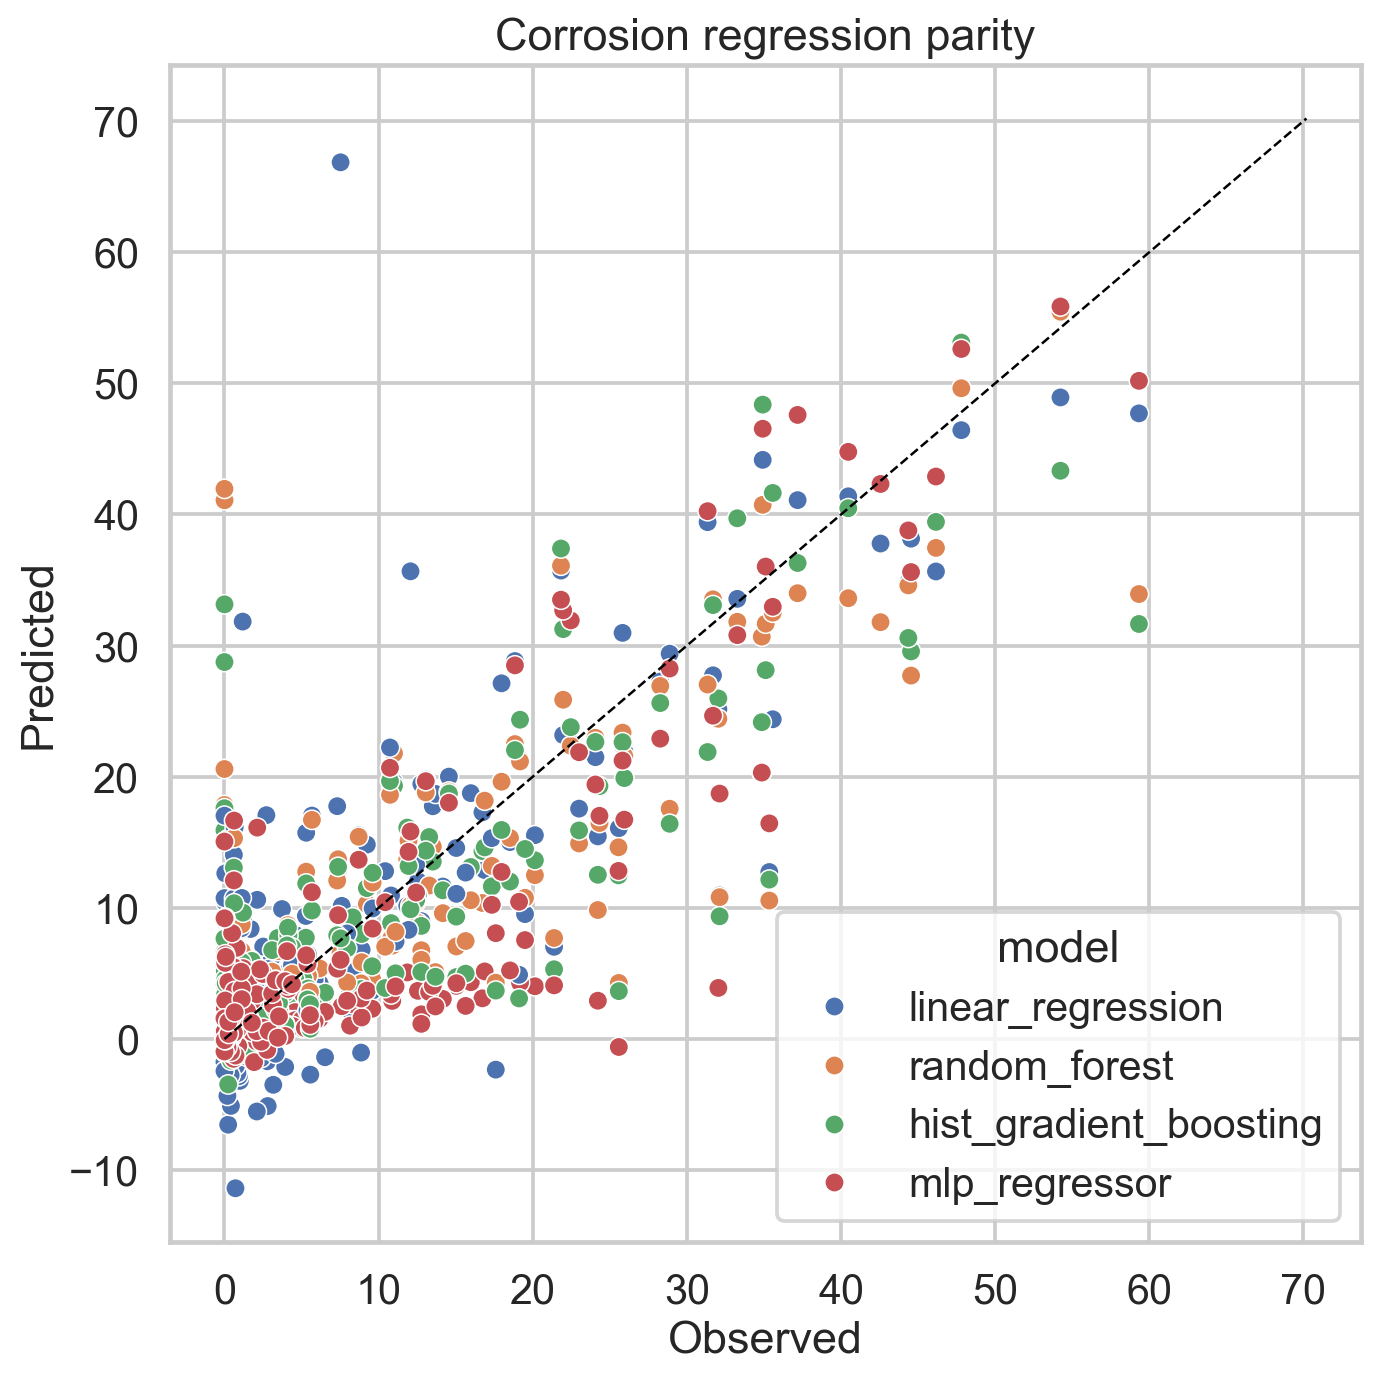
\includegraphics[width=0.86\textwidth]{reports/figures/corrosion_regression_parity.png}
\caption{Saved parity plot for corrosion regression under the \texttt{group\_shuffle} setting. This figure documents the strongest supported visible-corrosion result, not cross-campaign robustness.}
\label{fig:corrosion-parity}
\end{figure}

The visible-corrosion result does \emph{not} justify claiming that the model has learned internal structural damage, future failure time, or treatment-independent corrosion physics. It supports only current-state visible corrosion prediction under leakage-aware specimen holdout.

\subsection{Weak, Negative, and Mixed Results}

The damage stage is materially weaker than the corrosion stage. Even on \texttt{group\_shuffle}, the best saved mean \(R^2\) values are only 0.310 for wire loss and 0.385 for ultimate load. Once the holdout becomes campaign-based or treatment-based, average \(R^2\) becomes negative and, in the case of ultimate load, strongly negative. Those results do not support robust transport of hidden-damage estimation across campaigns or treatments.

\begin{figure}[H]
\centering
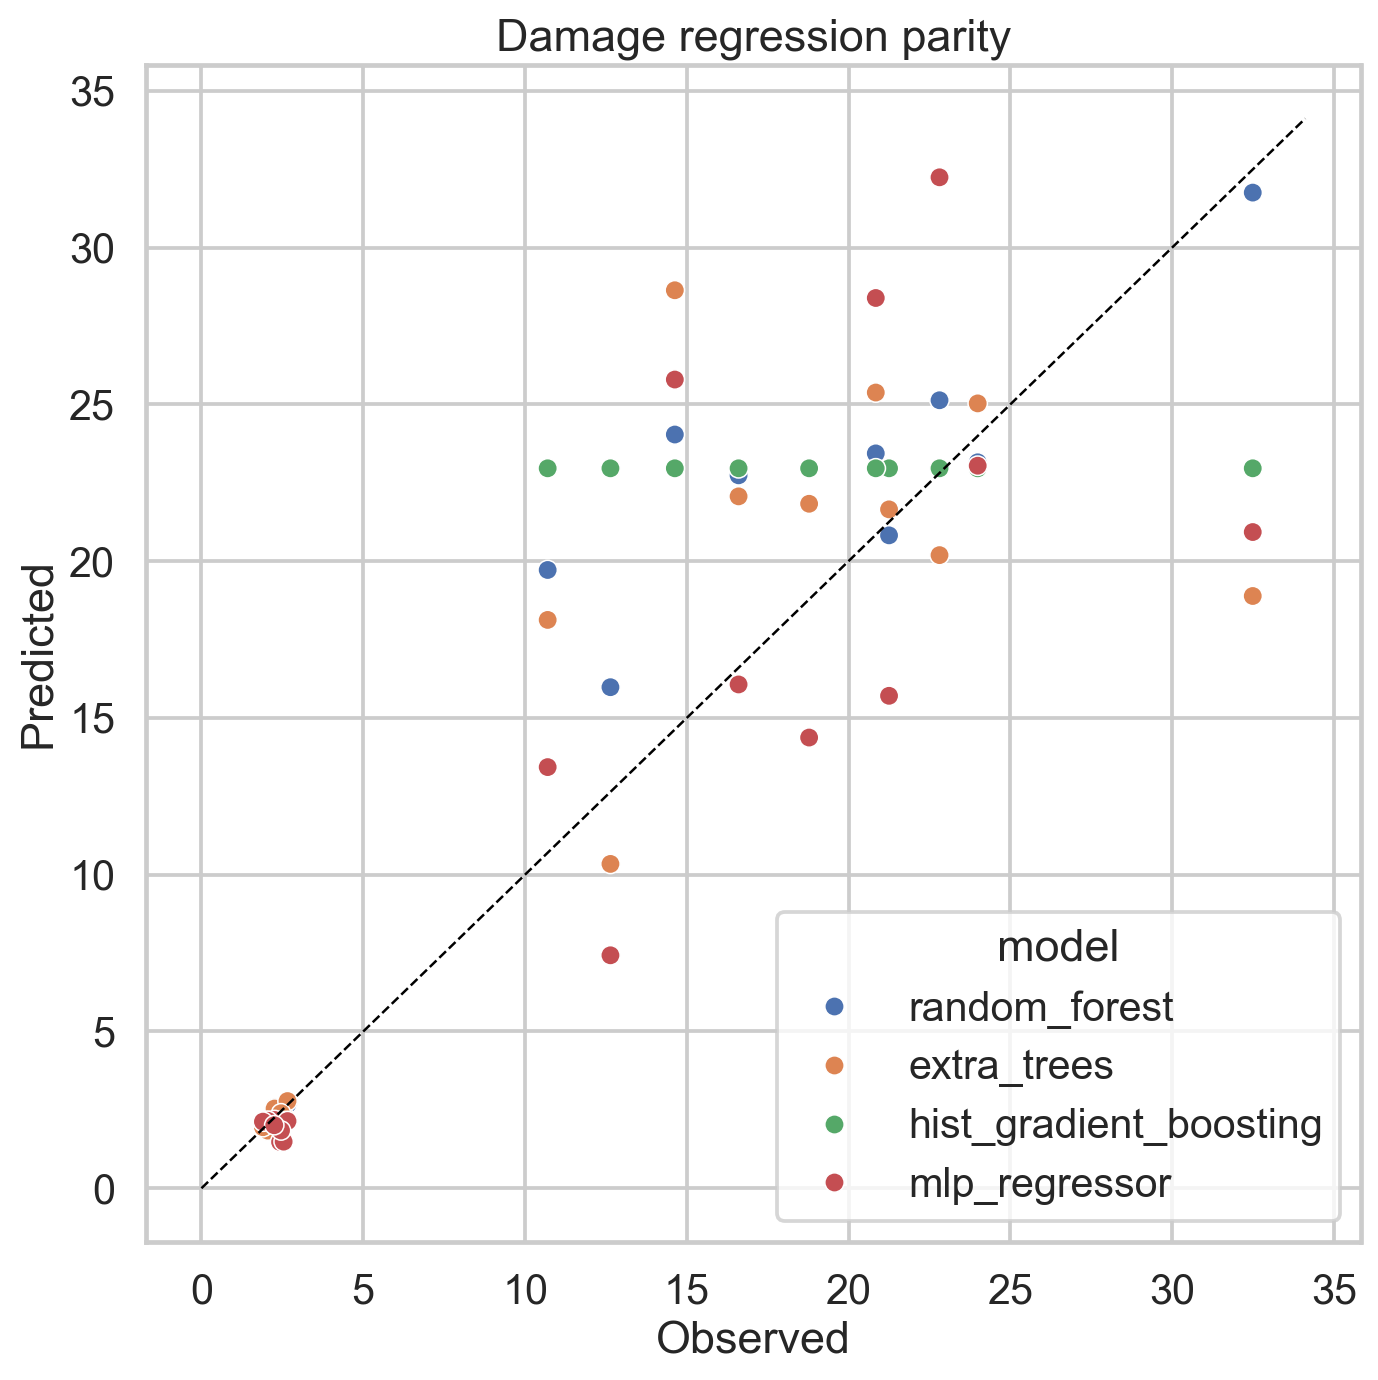
\includegraphics[width=0.86\textwidth]{reports/figures/damage_regression_parity.png}
\caption{Saved parity plot for damage regression under \texttt{group\_shuffle}. The plot is useful as an interpolation diagnostic only; it should not be read as cross-campaign or treatment-robust evidence.}
\label{fig:damage-parity}
\end{figure}

The saved full-data damage models also indicate that the two structural targets draw signal from different sources. For wire loss, the largest random-forest importances are \texttt{peak\_rust\_pct\_feature} (0.111), \texttt{cover\_failure\_surface\_mm} (0.093), \texttt{lab\_a\_mean} (0.081), \texttt{rust\_component\_count} (0.076), and manual \texttt{peak\_rust\_location\_cm} (0.075). For ultimate load, the leading importances are \texttt{n\_steel\_mesh} (0.172), both one-hot campaign indicators (0.128 and 0.105), \texttt{week} (0.101), \texttt{ageing\_days} (0.095), and \texttt{nacl\_pct} (0.082). This means the current load model is dominated by campaign-linked metadata rather than purely by image evidence.

The structural-label correlations reinforce that point. Across the 48 structural rows, \texttt{surface\_total\_rust\_pct} and \texttt{wire\_area\_loss\_pct} correlate only 0.021 overall, while \texttt{peak\_rust\_pct} and \texttt{wire\_area\_loss\_pct} correlate only 0.011. Meanwhile, \texttt{week}, \texttt{n\_steel\_mesh}, \texttt{ageing\_days}, and \texttt{nacl\_pct} are perfectly campaign-linked on the structural subset. The repository therefore supports only a weak claim that visible corrosion and selected image descriptors can help estimate hidden damage within the observed dataset; it does not support a strong claim that hidden damage is recoverable from images alone.

\subsection{Degradation and Proxy-RUL Outputs}

Surface corrosion curves fit observed repeated labels, so their in-sample fit is unsurprisingly good (median \(R^2\) about 0.903 for \texttt{surface\_total\_rust\_pct} and 0.916 for \texttt{peak\_rust\_pct}). However, the hidden-damage and load curves are fitted to model-generated estimates rather than repeated measurements. Piecewise-linear models dominate these fits, and the terminal forecast slopes are often flat or negative:
\begin{itemize}
  \item \texttt{estimated\_ultimate\_load\_kn}: 19 positive, 7 zero, 22 negative end slopes;
  \item \texttt{estimated\_wire\_area\_loss\_pct}: 10 positive, 32 zero, 6 negative end slopes.
\end{itemize}

This matters because degradation-to-threshold logic is sensitive to the forecast tail. A flat or negative tail can delay or remove a threshold crossing without any physical justification.

\begin{figure}[H]
\centering
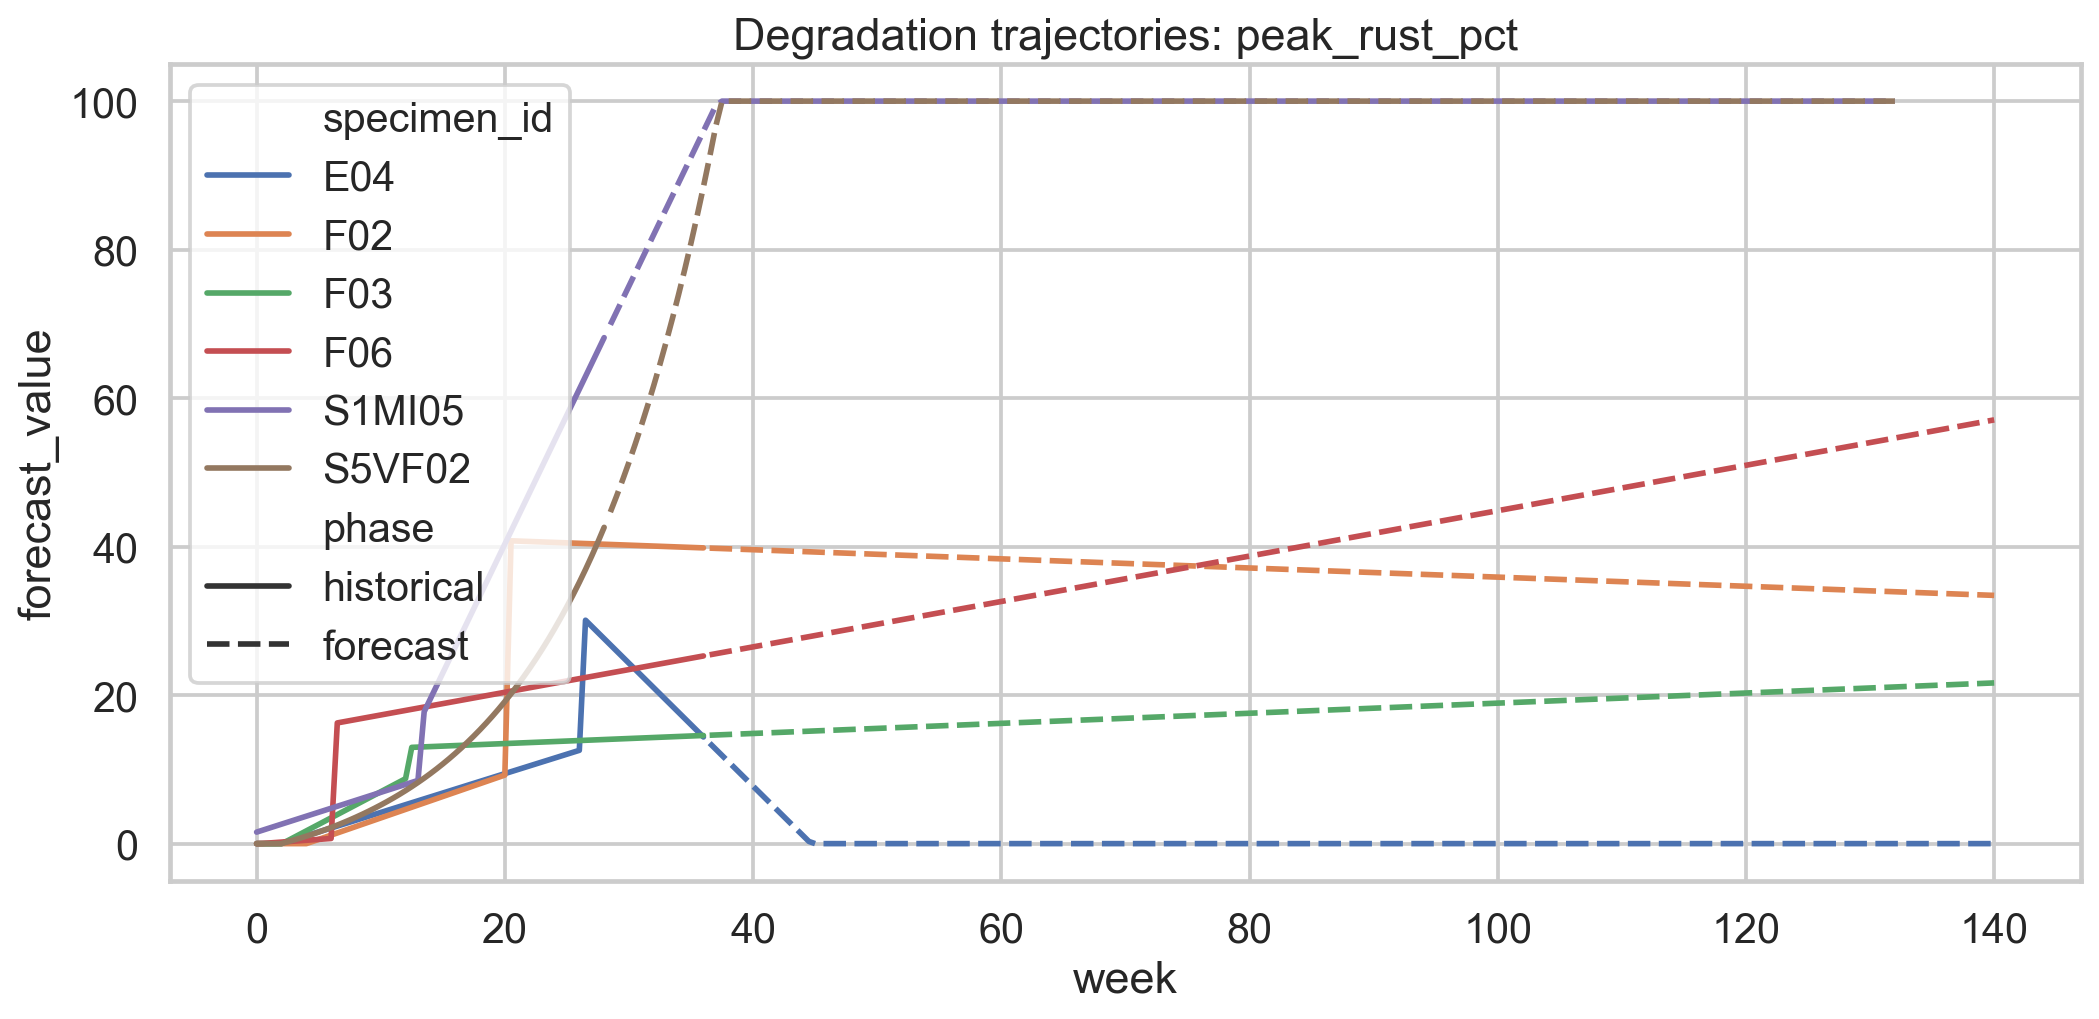
\includegraphics[width=0.88\textwidth]{reports/figures/degradation_examples_peak_rust.png}
\caption{Saved peak-rust trajectory examples for the highest proxy-risk specimens. These are specimen-wise fits and extrapolations, not ground-truth future observations.}
\label{fig:degradation-examples}
\end{figure}

\begin{table}[H]
\centering
\small
\begin{tabular}{lrrrP{4.2cm}}
\toprule
\textbf{Criterion} & \textbf{Finite rows} & \textbf{Zero-week rows} & \textbf{Median weeks} & \textbf{Interpretation} \\
\midrule
\texttt{rul\_wire\_20\_weeks} & 27 & 25 & 0.0 & Most specimens that ever cross the 20\% wire threshold are already at or beyond it in the latest saved state. \\
\texttt{rul\_wire\_25\_weeks} & 20 & 15 & 0.0 & This is one of the two governing criteria used in the final proxy RUL. \\
\texttt{rul\_wire\_30\_weeks} & 18 & 7 & 1.5 & Less immediately active than the 25\% threshold. \\
\texttt{rul\_load\_threshold\_weeks} & 27 & 15 & 0.0 & Often governs immediately when load margin is already small. \\
\texttt{rul\_health\_threshold\_weeks} & 10 & 0 & 24.0 & Rarely active and never the sole earliest governing criterion in the saved outputs. \\
\bottomrule
\end{tabular}
\caption{Threshold-crossing behavior in the saved proxy-RUL table.}
\label{tab:rul-thresholds}
\end{table}

The specimen-level proxy-RUL outputs are therefore exploratory and conservative in a specific way. Of the 48 specimens, 33 have a finite \texttt{estimated\_rul\_weeks}; among those finite values, 23 are exactly 0.0 weeks and the median is 0.0. Fifteen specimens never cross the chosen thresholds within the 104-week forecast horizon and remain missing. The governing-criterion counts are:
\begin{itemize}
  \item load only: 16 specimens;
  \item wire-loss 25\% only: 10 specimens;
  \item both wire-loss and load simultaneously: 7 specimens;
  \item no finite governing crossing within horizon: 15 specimens.
\end{itemize}

The health threshold is thus present in code but not materially active in the saved final proxy-RUL decision. The saved risk classes are 20 High, 8 Moderate, 20 Low, and 0 Critical. This is useful as a screening summary, but it does not justify the claim that the repository has learned true remaining life.

\section{What the Model Can and Cannot Learn}

\subsection{What Is Directly Visible}

The images directly contain visible rust color, rust spread, local concentration, texture changes, and edge-like deterioration patterns. The corrosion stage is therefore solving a problem that is physically present in the images. The best corrosion models are image-only and do not depend on treatment metadata.

\subsection{What Is Only Indirectly Inferable}

Wire-area loss and ultimate load are not directly visible in the images. At best, they can be inferred indirectly through correlations with surface corrosion, cover thickness, campaign conditions, and treatment history. The repository confirms this indirectness in two ways:
\begin{itemize}
  \item structural supervision exists only once per specimen and only at the end of observation;
  \item the saved hidden-damage models use metadata and manual corrosion labels, not just image-derived evidence.
\end{itemize}

This means the current damage stage is estimating latent structural state from a mixed evidence bundle, not discovering a purely image-based structural law.

\subsection{What Is Hidden and Not Reliably Recoverable Here}

True failure time is hidden and unrecoverable from the current dataset because it is never observed. More subtly, structural progression between week 0 and the final destructive test is also hidden: the dataset does not contain repeated direct measurements of wire loss or load capacity over time. The repository therefore fills that gap with model-generated hidden-damage estimates and then smooths them with curve fitting. That is a defensible exploratory engineering approximation, but it is not the same as observing hidden damage.

\subsection{Why Some Targets Are Easier Than Others}

Visible corrosion targets are easier because they are dense (792 labels), directly image-linked, and observed at every time point. Hidden-damage targets are harder because they are sparse (48 labels), terminal only, partially confounded with campaign, and physically not fully visible on the surface.

\subsection{Why Metadata Can Outperform Image Features}

In the structural subset, metadata fields encode campaign identity almost perfectly. For ultimate load, the saved full random forest draws most of its importance from mesh count, campaign indicators, week, ageing days, and NaCl level. In other words, the current model can partially exploit experimental design structure. Scientifically, that means metadata can look strong even when image-driven transportability is weak.

\subsection{Scientific Implication}

The most defensible scientific interpretation of \texttt{main\_3} is not ``images predict structural life.'' The stronger statement is: the repository demonstrates that visible corrosion state can be learned from images, and it assembles an exploratory condition-assessment stack that maps visible corrosion plus metadata to hidden-damage proxies and threshold-status indicators. That is useful, but it is not the same as validated structural prognosis.

\section{Traceability to the Original Thesis and Documentation}

The thesis chapter on automated image analysis and the conference paper both describe a method family that is related to \texttt{main\_3} but not identical to it. The thesis aligns with the current repository on the total number of images (792) and on the broad goal of color-based corrosion quantification. The conference paper reports 760 prepared images and a three-class classifier, so it corresponds to an earlier or narrower snapshot than the current repository.

\begin{longtable}{P{3.8cm}P{4.1cm}P{4.0cm}P{3.7cm}}
\caption{Traceability from documented thesis/conference methods to the current repository implementation.}\label{tab:traceability}\\
\toprule
\textbf{Documented method element} & \textbf{What the documentation says} & \textbf{What the repository actually does} & \textbf{Expected consequence of mismatch} \\
\midrule
\endfirsthead
\toprule
\textbf{Documented method element} & \textbf{What the documentation says} & \textbf{What the repository actually does} & \textbf{Expected consequence of mismatch} \\
\midrule
\endhead
\midrule
\multicolumn{4}{r}{Continued on next page} \\
\endfoot
\bottomrule
\endlastfoot
Preprocessing toolchain & Thesis chapter 7 describes manual and batch GIMP/BIMP preprocessing with resize to 3555\(\times\)886 px, crop to 2835\(\times\)650 px, and white-balance level adjustment using input range \([0,195]\) and output \([0,255]\) & \texttt{main\_3} loads the existing PNG files, crops by relative ratios, rescales channel intensities by percentiles, and uses adaptive histogram equalization in Python & Color and geometry normalization are not thesis-equivalent. Any mismatch in feature-target alignment can partly arise from preprocessing differences. \\
Segmentation logic & Thesis and conference paper describe MATLAB RGB thresholding with rust mask \([25,0,0]\) to \([255,100,80]\) plus explicit black-pore and gray-mark exclusion masks & \texttt{main\_3} uses a weighted RGB/HSV/Lab rust-likelihood score, adaptive thresholding, and morphology cleanup & The current mask is more adaptive but less directly traceable to the documented thresholds. Quantitative agreement with thesis overlays cannot be assumed. \\
Spatial strip analysis & Thesis describes 1 cm strip analysis with overlap, averaging about 47 strips over a 24 cm specimen; conference paper mentions 0.5 cm strips & \texttt{main\_3} uses 12 non-overlapping longitudinal segments over 24 cm & Current spatial features are coarser and structurally different from both documented strip schemes. Direct equivalence of peak-location or peak-rust calculations is unsupported. \\
Target formulation & Conference paper trains a three-class low/medium/high corrosion classifier; thesis discussion centers on segmented rust area and strip peaks & \texttt{main\_3} trains regressors for spreadsheet corrosion percentages and classifiers for spreadsheet 1--5 category labels & The repository is solving a different supervised task from the documented three-class classifier, even though the physical topic is related. \\
Learning model & Conference paper describes transfer learning on ResNet-50 & \texttt{main\_3} uses handcrafted feature extraction plus classical ML; the older deep baseline is in sibling project \texttt{main\_2}, not in the saved \texttt{main\_3} pipeline & Reported \texttt{main\_3} results should not be presented as direct reproduction of the documented ResNet workflow. \\
Automation artifacts & Thesis states that full MATLAB code and GIMP/BIMP configuration exist as attachments & Those exact MATLAB and BIMP source files are not present in \texttt{main\_3}; only the current Python reimplementation is available & Exact thesis preprocessing and mask-generation reproducibility cannot be verified from the repository alone. \\
Dataset provenance & Conference paper states 760 prepared images; thesis states 792 preprocessed images & Current repository contains 792 rows and 792 PNGs, matching the thesis count & The current repository is closer to the thesis dataset snapshot than to the conference snapshot, but the snapshots are not perfectly interchangeable. \\
\end{longtable}

The traceability conclusion is therefore mixed. The current repository is clearly thesis-inspired in its use of corrosion-focused image analysis and strip-like localization logic, but it is not an exact code reproduction of the thesis GIMP+MATLAB workflow. The current implementation should be described as a Python reconstruction and extension, not as exact reproduction.

\section{Limitations}

The limitations are not generic; they are tied directly to the present repository state.

\begin{itemize}
  \item \textbf{Small structural supervision.} Only 48 rows carry structural labels, and each specimen contributes exactly one structural row. This is the dominant bottleneck.
  \item \textbf{Campaign dependence.} The two campaigns differ simultaneously in week horizon, mesh count, NaCl level, ageing days, and treatment composition. Several metadata fields become campaign surrogates.
  \item \textbf{Treatment imbalance.} Structural rows per treatment are highly uneven, from 2 rows for \texttt{VF} and 2 for \texttt{SA\_VF} up to 18 for \texttt{SA}. Leave-one-treatment-out damage regression is therefore very unstable.
  \item \textbf{No direct RUL supervision.} The dataset contains no failure times, no censoring labels, and no experimentally observed end-of-life events, so only threshold-based proxy RUL is possible.
  \item \textbf{Downstream manual-label dependence.} Hidden-damage estimation is not end-to-end image-only because manual corrosion labels are used as damage-model inputs.
  \item \textbf{Model-on-model trajectories.} Hidden-damage and load degradation curves are fitted to model estimates at all weeks rather than to repeated structural measurements.
  \item \textbf{No monotonicity constraint.} The curve fitting can produce flat or negative progression rates, especially for hidden-damage proxies and load.
  \item \textbf{Preprocessing uncertainty.} The thesis workflow described in documentation is not exactly reproduced. This likely contributes to the weak direct correlation between intuitive mask-based proxies and the manual corrosion labels.
  \item \textbf{Category-definition ambiguity.} The repository stores ordinal corrosion categories but does not define the quantitative cutoffs behind the 1--5 scale.
  \item \textbf{Single corrupted image retained.} One unreadable PNG remains in the dataset with a failure flag and median-filled features. This is minor globally but real.
  \item \textbf{External validity.} The saved models are calibrated only on 48 ferrocement specimens across two campaigns. Generalization beyond that regime is untested.
\end{itemize}

\section{Future Work}

Only follow-up work that directly addresses the observed weaknesses is justified.

\begin{itemize}
  \item Recover or reimplement the exact thesis preprocessing attachments (GIMP/BIMP settings and MATLAB masks) and quantify feature-level agreement against the current Python pipeline.
  \item Separate the downstream damage stage into explicit ablations: metadata-only, manual-corrosion-only, image-only, and mixed-input models. The current repository cannot isolate these contributions.
  \item Generate out-of-fold hidden-damage estimates for all rows before fitting degradation curves, so that downstream trajectory fitting does not rely on in-sample refits over the same structural labels.
  \item Collect repeated structural measurements before the destructive endpoint. Even a small number of intermediate wire-loss or load observations would materially improve damage progression modeling.
  \item Add monotone or physics-informed trajectory constraints for wire loss and residual capacity, because the current best-RMSE fits frequently flatten or reverse at the forecast tail.
  \item Define and document the 1--5 corrosion-category rules in the repository, or replace them with transparent threshold labels derived from explicit numeric rules.
  \item Build a specimen-treatment mapping table that decouples series naming from treatment identity, so future analyses cannot accidentally infer treatment from filenames.
  \item Validate the threshold-based RUL outputs against experimentally observed threshold crossings in future campaigns, rather than only against model-generated forecasts.
\end{itemize}

\appendix

\section{Meeting-Defense Questions and Concise Evidence-Based Answers}

\paragraph{Why not direct RUL?}
Because neither the spreadsheet nor the outputs contain true failure times. The repository only has current corrosion labels at every image and structural labels at one late-stage row per specimen. The saved \texttt{estimated\_rul\_weeks} value is therefore a threshold-crossing time computed from forecasted states, not a supervised failure-time target.

\paragraph{Why these split strategies?}
Random row-wise splitting would leak different weeks of the same specimen across train and test. \texttt{group\_shuffle} prevents that by holding out whole specimens. Leave-one-treatment-out and leave-one-campaign-out are stricter stress tests that expose domain dependence and shortcut learning.

\paragraph{Why did robustness drop under stricter holdouts?}
Because the data-generating conditions change with treatment and especially with campaign. In the structural subset, week, mesh count, ageing days, and NaCl level are effectively campaign markers. Once those markers are held out, performance collapses, especially for hidden-damage targets.

\paragraph{Why can visible corrosion be predicted better than structural degradation?}
Visible corrosion is directly present in the images and has 792 supervised rows. Structural degradation is only sparsely observed, is mostly hidden beneath the surface, and has only 48 late-stage labels.

\paragraph{How much of the downstream signal comes from metadata?}
The repository does not contain a clean ablation study, so the exact fraction cannot be recovered from saved outputs alone. However, the saved full ultimate-load random forest is dominated by metadata and campaign indicators, which is strong evidence that metadata contributes materially.

\paragraph{Are the corrosion results partly tautological?}
Partly, in the sense that the features were engineered to respond to rust-colored regions. But the current Python features are not numeric copies of the manual labels: \texttt{rust\_area\_pct\_feature} correlates only 0.257 with \texttt{surface\_total\_rust\_pct}, and \texttt{peak\_rust\_pct\_feature} correlates only 0.183 with \texttt{peak\_rust\_pct}. So the model is not simply reading back an identical mask.

\paragraph{Could preprocessing mismatch explain part of the failure?}
Yes. The thesis documents a GIMP/BIMP plus MATLAB RGB-threshold workflow, while \texttt{main\_3} uses a Python adaptive-color pipeline. That mismatch is a plausible explanation for why intuitive area/peak proxies align only weakly with the manual corrosion labels.

\paragraph{What are the highest-risk assumptions in the repository?}
The highest-risk assumptions are: scaling raw wire-loss values by 100, treating hidden-damage trajectories as smooth fits to model-generated estimates, and using campaign-linked metadata inside structural proxy models without a clean causal disentangling step.

\paragraph{Which features are currently the most interpretable?}
The most interpretable families are the rust-mask area, segment-wise rust distribution, peak-rust location, connected-component geometry, and color statistics. They can be tied to visible surface patterns. Their weakness is that they are sensitive to segmentation quality and preprocessing consistency.

\paragraph{What exactly do the important metrics mean?}
\texttt{MAE} is mean absolute error in target units. \texttt{RMSE} penalizes larger errors more strongly. \(R^2\) measures explained variance and can become negative when the model is worse than predicting the mean. \texttt{Macro-F1} averages per-class F1 scores and is more reliable than accuracy under class imbalance. \texttt{progression\_rate\_per\_week} is the final forecast slope of a fitted curve. \texttt{health\_index} is a weighted score from corrosion, wire loss, and load margin. \texttt{failure\_probability} is only a proxy risk score. \texttt{estimated\_rul\_weeks} is weeks to the earliest selected threshold crossing, not weeks to true failure.

\paragraph{What is the shortest defensible description of the whole system?}
\texttt{main\_3} is a repository-grounded corrosion-to-threshold-status pipeline. It gives credible image-based visible corrosion estimates for unseen specimens under related conditions, but hidden-damage estimation and proxy RUL remain exploratory because the structural supervision is sparse, campaign-linked, and not true failure-time data.

\end{document}
